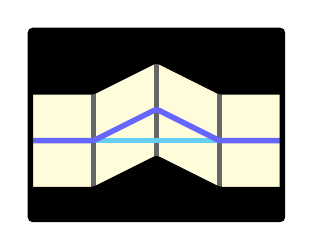
\begin{tikzpicture}[thick,scale=0.4, every node/.style={scale=0.4}]

\tikzset{cross/.style={thick, cross out, line width=4, minimum size=10pt, inner sep=0pt, outer sep=0pt},
%default radius will be 1pt. 
cross/.default={1pt}}

\begin{scope}

\clip (0,0) -- (8,0) -- (8,6) -- (0,6) -- cycle;

\draw [line width=0,fill=yellow!15!white] (0,0) -- (8,0) -- (8,6) -- (0,6) -- cycle;

\draw [black!60!white,line width=2,line cap=round] (2,1) -- (2,4);
\draw [black!60!white,line width=2,line cap=round] (4,2) -- (4,5);
\draw [black!60!white,line width=2,line cap=round] (6,1) -- (6,4);

\draw [fill=black,rounded corners=1] (0,0) -- (0,1) -- (2,1) -- (4,2) -- (6,1) -- (8,1) -- (8,0) -- cycle;
\draw [fill=black,rounded corners=1] (0,6) -- (0,4) -- (2,4) -- (4,5) -- (6,4) -- (8,4) -- (8,6) -- cycle;

\draw [cyan!60!white,line width=2,line cap=round,rounded corners=1] (2,2.5) -- (6,2.5);
\draw [blue!60!white,line width=2,line cap=round,rounded corners=1] (0,2.5) -- (2,2.5) -- (4,3.5) -- (6,2.5) -- (8,2.5);

\end{scope}

\draw [line width=2,rounded corners=1] (0,0) -- (8,0) -- (8,6) -- (0,6) -- cycle;

\end{tikzpicture}